\documentclass[ngerman]{article}
\usepackage[a4paper]{geometry}
\usepackage{babel}
\usepackage{graphicx}
\usepackage{hyperref}
\usepackage{cleveref}

\title{
    
\includegraphics[width=3cm]{assets/icon.png}\\
    \textbf{Multimodal Parliament Explorer - Projektdokumentation}
}
\author{
    Kai Wöllstein
    \and Philipp Schneider
    \and Philipp Hein
    \and Philipp Landmann}


\date{\today}

\begin{document}


    \maketitle
    \tableofcontents
    \newpage

    \section{Kurze Vorstellung des Projektes}

    Unser Abschlussprojekt - Multimodaler Parlament Explorer - ist eine Applikation, mit der man die vielen verschiedenen Reden im deutschen Bundestag visualisieren und analysieren kann.

    Die Informationen dafür sind aus verschiedenen Quellen zusammengetragen und wir bieten den Mehrwehrt, diese Informationen möglichst übersichtlich und nützlich darzustellen.

    \subsection{Screenshots}

    \begin{figure}[h]
        \centering
        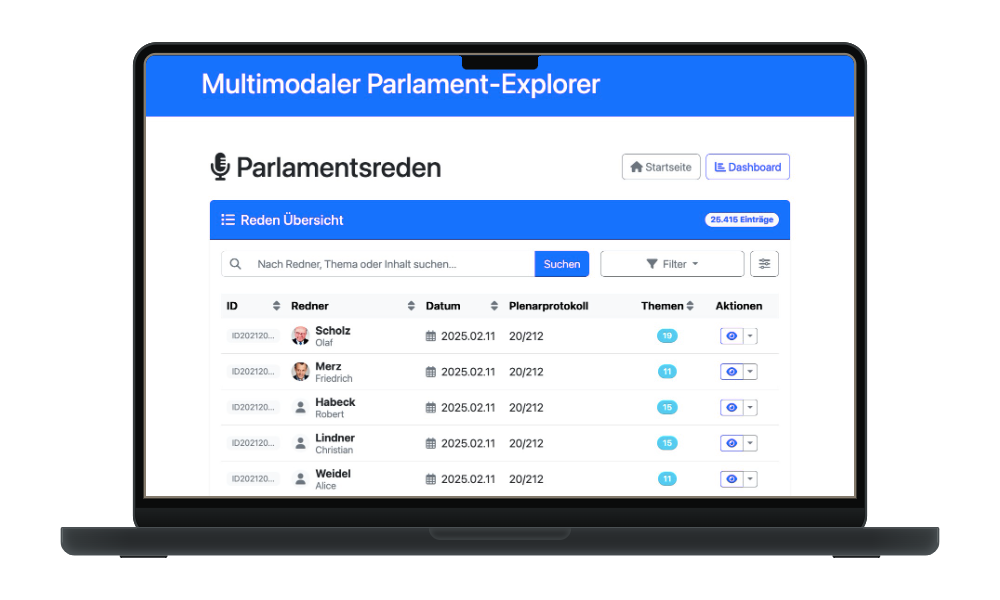
\includegraphics[width=0.9\linewidth]{assets/screenshot-1.png}
        \caption{Screenshot 1}
        \label{fig:screenshot-1}
    \end{figure}

    \begin{figure}[h]
        \centering
        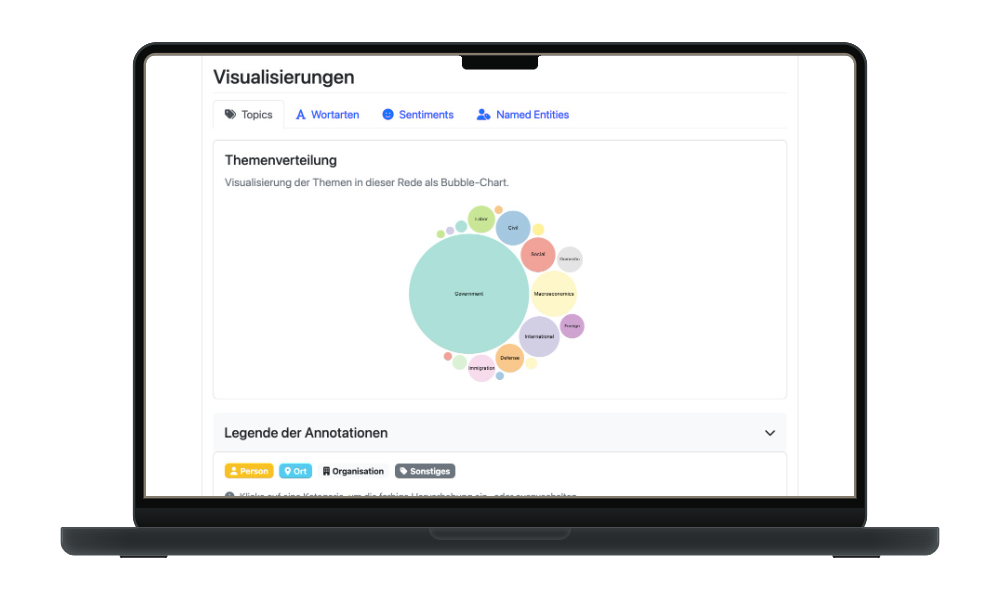
\includegraphics[width=0.9\linewidth]{assets/screenshot-2.png}
        \caption{Screenshot 2}
        \label{fig:screenshot-2}
    \end{figure}

    \newpage
    \subsection{Techstack}

    \begin{itemize}
        \item \textbf{Java 17} im Backend
        \item \textbf{Javalin} als Webserver
        \item \textbf{Freemarker} als Templating-Engine
        \item \textbf{MongoDB} als Datenbank
        \item \textbf{D3.js / TikZ} zum Generieren von Diagrammen
    \end{itemize}

    \section{Organisation des Projektes}

    \subsection{Aufteilung in Module}

    Damit wir möglichst effektiv an dem Projekt arbeiten und möglichst schnell vorankommen, haben wir direkt am Anfang die Aufgabenstellung in mehrere Teile aufgeteilt und diese folgendermaßen untereinander im Team aufgeteilt:

    \begin{itemize}
        \item \textbf{Diagramme} Philipp Hein
        \item \textbf{Backend} Philipp Hein, Philipp Schneider
        \item \textbf{NLP} Kai Wöllstein
        \item \textbf{Frontend} Philipp Schneider
        \item \textbf{Dokumentation} Philipp Landmann
    \end{itemize}

    Natürlich ist die Zuteilung einigermaßen flexibel gehalten; einige Bereiche können sich überlappen, bzw. man kann auch in anderen Bereichen als dem eigenen Hauptbereich tätig werden.

    \subsection{Nutzung von Tickets / Issues}

    Um die Übersicht über die vielen Teilaufgaben zu behalten, haben wir extensiv GitLab-Issues genutzt.
    Damit konnten wir einfach sehen, wie weit wir schon sind und was noch zu tun ist, bzw. entstandene Deadlocks erkennen.

    Besonders bei den Issue-Boards kann man sehen, wie viele Issues pro Person noch gelöst werden müssen.

    \subsection{Kommunikation im Team}

    Die Kommunikation im Team wurde mit einer ca. wöchentlichen Videokonferenz gelöst, in der wir besprechen, was wir als nächstes machen und was wir bisher schon erreicht haben.

    Zusätzlich hatten wir eine WhatsApp-Gruppe, sowie die GitLab Issues als Kommunikationskanäle.

    \section{Projektverlauf und Dokumentation der Eigenleistungen}

    \begin{figure}
        \centering
        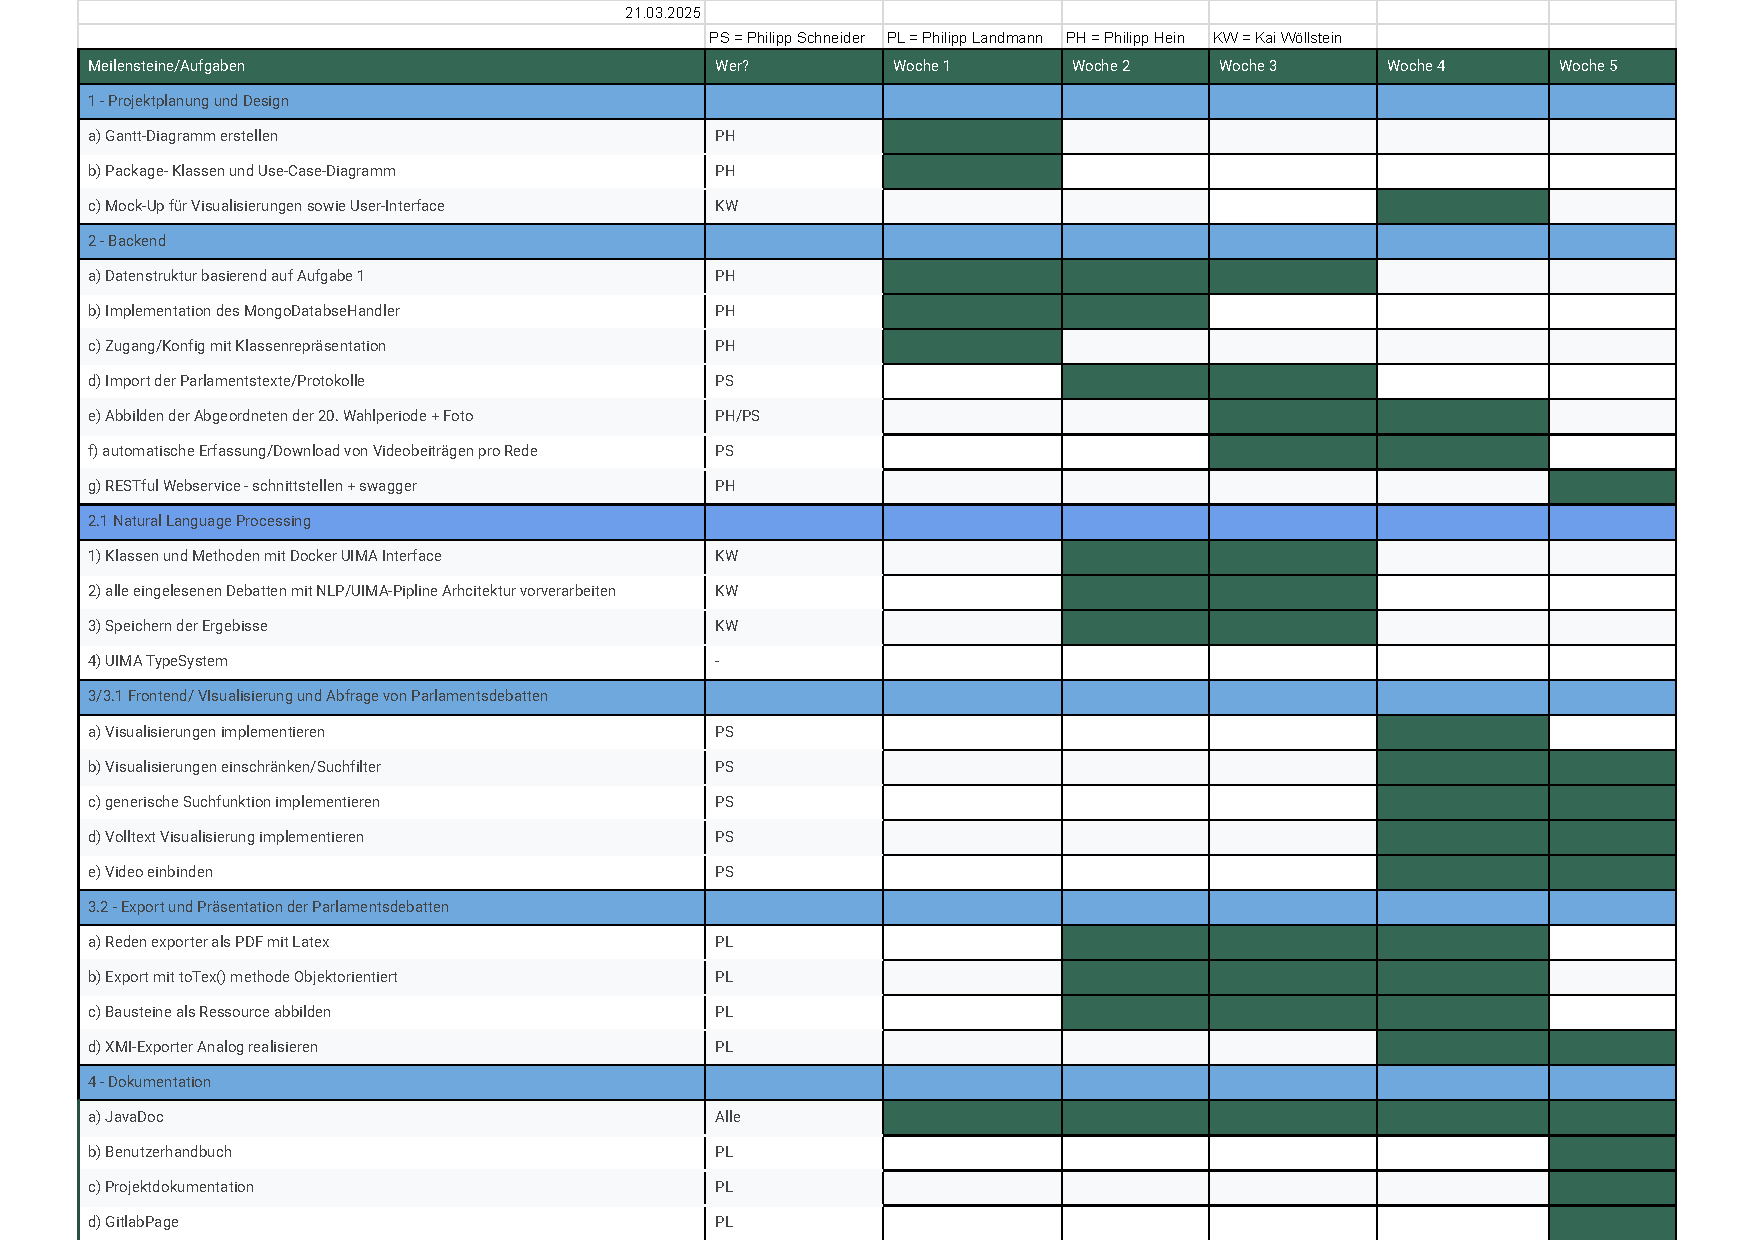
\includegraphics[width=\linewidth]{assets/gantt-diagramm.pdf}
        \caption{Projektverlauf - als Gantt-Diagramm dargestellt}
        \label{fig:gantt-dia}
    \end{figure}

    In \Cref{fig:gantt-dia} sieht man ein Gantt-Diagramm des Projektverlaufs.
    Man kann erkennen - Die Aufgaben sind ziemlich gleichmäßig auf die Gruppe aufgeteilt, und die Zuteilung, die wir am Anfang getroffen haben, hat sich bestätigt.

\end{document}
